\part{Z変換}
	\chapter{基礎理論}
		\section{最終値定理}
			\begin{shadebox}
				$X(z)\;(z\in\complexNumbers)$を離散時間信号$x(n)\;(n \in \integers,\;\forall n<0,x(n)=0)$のZ変換とする。
				$\lim_{n\to\infty} x(n)$が存在するとき次が成り立つ。
				\[ \lim_{z\to1}(z-1)F(z) = \lim_{n\to\infty} x(n) \]
				但し上式に於ける$\lim_{z\to1}$では$z$が実軸上で右側から1に近づくことを意味する。
			\end{shadebox}
			\begin{proof}
				\quad\par
				$\alpha = \lim_{n\to\infty} x(n)$とする。
				発想としては、十分大きい$N\in\naturalNumbers$に対して$\sum_{k=N+1}^\infty x(k)z^{-k} \sim \sum_{k=N+1}^\infty \alpha z^{-k} = \alpha z^{-N}\frac{1}{z-1}$となることを利用する。
				\par
				任意の$\varepsilon \in (0,1)$に対してある$N\in\naturalNumbers$が存在して$\forall n\geq N,\;|x(n)-\alpha|<\varepsilon$となる。
				\begin{align}
					\quad &\lim_{z\to1}(z-1)F(z) - \alpha = \lim_{z\to1}(z-1)z^N F(z) - \alpha \nonumber \\
					&= \lim_{z\to1}(z-1)z^N\left(\sum_{k=0}^{N-1} x(k)z^{-k} + \sum_{k=N+1}^\infty x(k)z^{-k}\right) - (z-1)z^N\sum_{k=N+1}^\infty \alpha z^{-k} \nonumber \\
					&= \lim_{z\to1}(z-1)z^N \sum_{k=N+1}^\infty (x(n) - \alpha)z^{-k} \quad \left(\sum_{k=0}^{N-1}\text{の項は極限で消える}\right) \\
					|(1)| &\leq \lim_{z\to1}(z-1)z^N \sum_{k=N+1}^\infty |x(n) - \alpha|z^{-k} < \lim_{z\to1}(z-1)z^N \sum_{k=N+1}^\infty \varepsilon z^{-k} = \varepsilon \nonumber
				\end{align}
			\end{proof}
		\section{複素指数関数入力に対する伝達関数の作用}
			\begin{shadebox}
				$A>0,\;\omega \in \realNumbers$とする。
				離散時間信号$x: \realNumbers \to \complexNumbers$を次のように定める。
				\[
					x(n) =
					\begin{cases}
						Ae^{i\Omega n} & (n\geq 0) \\
						0 & (n<0)
					\end{cases}
				\]
				$H: z\in\complexNumbers \mapsto H(z) \in \complexNumbers$を、$1/z$を変数とした有理式として既約であるような有理関数とする。
				また、$H$の極の絶対値は全て1未満であるとする。
				伝達関数が$H(z)$である離散時間システムに信号$x$を入力した時の出力を$y$とすると、十分大きい$n$に対して
				$y(n) \sim H(\NapierE^{i\Omega})x(n)$となる。
			\end{shadebox}
			\begin{proof}
				\quad\par
				$N_\text{p}$を$H(s)$の相異なる極の個数とし、それら極を$p_0,\dots,p_{N_\text{p}}$とする。
				極$p_k$の次数を$N_{\text{p},k}$とし、$H(z)$の部分分数展開を
				\[ H(z) = c_0 + \sum_{k=1}^{N_\mathrm{p}} \sum_{l=1}^{N_{\mathrm{p},k}} \frac{c_{k,l}}{(1-p_kz^{-1})^l} \]
				とする。
				ここに$c_0,c_{k,l}\;(k=1,\dots,N_\mathrm{p},l=1,\dots,N_{\mathrm{p},k})$は適当な複素数である。
				$x,y$のZ変換をそれぞれ$X,Y$とすると$Y(z) = H(z)F(z) = A H(z)/(1-\NapierE^{i\Omega}z^{-1})$である。
				これの部分分数展開に現れる、$1/(1-p_k z^{-1})^l\;(k=1,\dots,N_\mathrm{p},l=1,\dots,N_{\mathrm{p},k})$に比例する項は逆Z変換すると$n$の多項式と公比$p_k$の等比級数の積となり、$n\to\infty$で0に収束する。
				(このことはZ変換の性質: 時間シフト$\mathcal{Z}[x(n+k)] = z^kX(z)$、およびZ領域微分$\mathcal{Z}[nx(n)] = -z\derivLong{\mathcal{Z}[x(n)]}{z}{}$を繰り返し用いることで分かる)
				\par
				残りの項、すなわち$1/(1-\NapierE^{i\Omega}z^{-1})$に比例する項は$AH(\NapierE^{i\Omega})/(1-\NapierE^{i\Omega}z^{-1}) = H(\NapierE^{i\Omega})X(z)$となる。
			\end{proof}
	\chapter{IIRフィルタの計算手順}
		\begin{figure}[H]
			\centering
			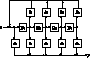
\includegraphics[keepaspectratio, scale=5]
			{parts/Z-transform/imgs/IIR-filter/calculationMethod/blockDiagram.pdf}
			\caption{IIRフィルタのブロック図の例}
		\end{figure}
		上の例で示したIIRフィルタの出力は以下の手続きで計算できる(仕事で関わっていたデジタル無線機の信号処理部でそうやっていた)。
		\begin{enumerate}
			\item $D_1,\cdots D_4 \leftarrow 0$
			\item $n \leftarrow 0$
			\item $\alpha \leftarrow a_1D_1 + \cdots a_4D_4$
			\item $\beta \leftarrow b_1D_1 + \cdots b_4D_4$
			\item $\gamma \leftarrow x(n) + \beta$
			\item $y(n) \leftarrow \alpha + a_0\gamma$
			\item $D_4 \leftarrow D_3,\;D_3 \leftarrow D_2,\;D_2 \leftarrow D_1,\;D_1 \leftarrow \gamma$
			\item $n \leftarrow n+1$
			\item $n$が$x$の定義域の末尾に達しているなら終了。そうでないなら3に戻る。
		\end{enumerate}